\documentclass[12pt,a4paper]{article}
\usepackage[utf8]{vietnam}
\usepackage{amsmath,amssymb}
\usepackage{tabularx}
\usepackage{tikz}
\usepackage{xcolor}
\usepackage[top=0.6cm, bottom=0.6cm, left=0.6cm, right=0.6cm]{geometry}
\usepackage[dethi]{ex_test}

\SAOPTN{widthSA=3.2,heightSA=0.62}
\setlength{\parskip}{0pt}

% Dong ke cham mo chuan viet tay
\newcommand{\dongke}[1]{%
  \begingroup%
  \setlength{\parskip}{0pt}%
  \baselineskip=18.5pt%
  \vspace{1.0mm}%
  \foreach \i in {1,...,#1}{%
    \noindent{\color{gray!60}\dotfill}\par%
  }%
  \vspace{0.6mm}%
  \endgroup%
}

% Dinh nghia o bai tap tu luan trong bang
\newcommand{\oBaiTap}[3][6]{%
  \vspace{1.0mm}%
  \noindent\textbf{#2} #3\par%
  \dongke{#1}%
}

\begin{document}
\pagestyle{empty}
% =============================================================================
% ========================= TOAN 9 TUAN 09 BUOI 02 - MA DE 101 =================
% ========================= TRANG 1/2 ==========================================
% =============================================================================
\noindent
\begin{tabularx}{\linewidth}{|X|c|}
\hline
\textbf{PHIẾU KIỂM TRA ĐỊNH KỲ TOÁN 9 - TUẦN 09 - BUỔI 02} & \textbf{Mã đề: 101 - Trang 1/2} \\
\hline
\end{tabularx}

\vspace{1.0mm}

\noindent
\begin{tabularx}{\linewidth}{|p{3.2cm}|X|}
\hline
\centering\textbf{ĐIỂM SỐ} & \centering\textbf{LỜI NHẬN XÉT CỦA THẦY CÔ} \tabularnewline
\hline
\rule{0pt}{1.8cm} & \tabularnewline
\hline
\end{tabularx}

\vspace{1.2mm}
\noindent\textbf{Câu 1 (0,25 điểm).} Tâm đối xứng của đường tròn $(O; R)$ là điểm nào?: \shortans{Tâm O}\par\vspace{0.6mm}
\noindent\textbf{Câu 2 (0,25 điểm).} Trục đối xứng của một đường tròn là đường thẳng nào?: \shortans{Mọi đường kính}\par\vspace{0.6mm}
\noindent\textbf{Câu 3 (0,25 điểm).} Đường kính vuông góc với một dây cung thì có tính chất gì?: \shortans{Đi qua trung điểm dây}\par\vspace{0.6mm}
\noindent\textbf{Câu 4 (0,25 điểm).} Cho $(O; 10\text{ cm})$, dây $AB = 16\text{ cm}$. Khoảng cách từ tâm $O$ đến dây $AB$ là: \shortans{6\text{ cm}}\par\vspace{0.6mm}
\noindent\textbf{Câu 5 (0,25 điểm).} Cho $(O; 5\text{ cm})$, khoảng cách từ tâm $O$ đến dây $CD$ là $3\text{ cm}$. Dây $CD$ dài: \shortans{8\text{ cm}}\par\vspace{0.6mm}
\noindent\textbf{Câu 6 (0,25 điểm).} Kết quả rút gọn biểu thức $\sqrt{(3 - 2\sqrt{2})^2}$ bằng: \shortans{3 - 2\sqrt{2}}\par\vspace{0.6mm}
\noindent\textbf{Câu 7 (0,25 điểm).} Trục căn thức ở mẫu của biểu thức $\dfrac{2}{\sqrt{3}-1}$ được kết quả là: \shortans{\sqrt{3}+1}\par\vspace{0.6mm}
\noindent\textbf{Câu 8 (0,25 điểm).} Nghiệm của phương trình $\sqrt{x - 3} = 4$ là $x = $: \shortans{19}\par\vspace{0.6mm}
\noindent\textbf{Câu 9 (0,25 điểm).} Nghiệm của hệ phương trình $\begin{cases} 2x + 3y = 7 \\ 2x - 3y = 1 \end{cases}$ là $(x; y) = $: \shortans{(2; 1)}\par\vspace{0.6mm}
\noindent\textbf{Câu 10 (0,25 điểm).} Vòm tròn bán kính $5\text{ m}$. Bề rộng mặt đường cách đỉnh vòm $1\text{ m}$ là: \shortans{6\text{ m}}\par\vspace{0.6mm}
\vspace{0.8mm}
\noindent\textbf{Câu 11 (2,5 điểm). Đại số tổng hợp:}
\vspace{0.6mm}

\noindent
\begin{tabularx}{\linewidth}{|X|X|}
\hline
\oBaiTap[20]{a) (1,25 điểm)}{Giải hệ phương trình:\par $\begin{cases} 3(x - 1) + 2y = 5 \\ 2x - (y + 1) = 2 \end{cases}$} & 
\oBaiTap[20]{b) (1,25 điểm)}{Cho biểu thức với $x > 0, x \ne 1$:\par $Q = \left(\dfrac{\sqrt{x}+1}{\sqrt{x}-1} - \dfrac{\sqrt{x}-1}{\sqrt{x}+1}\right) : \dfrac{4\sqrt{x}}{x-1}$\par Rút gọn biểu thức $Q$.} \\
\hline
\end{tabularx}

\newpage
% =============================================================================
% ========================= TOAN 9 TUAN 09 BUOI 02 - MA DE 101 =================
% ========================= TRANG 2/2 ==========================================
% =============================================================================
\noindent
\begin{tabularx}{\linewidth}{|X|c|}
\hline
\textbf{TOÁN 9 - TUẦN 09 - BUỔI 02} & \textbf{Mã đề: 101 - Trang 2/2} \\
\hline
\end{tabularx}

\vspace{1.2mm}

\noindent
\begin{tabularx}{\linewidth}{|X|}
\hline
\vspace{0.5mm}
\textbf{Câu 12 (2,5 điểm).} Hai ô tô khởi hành cùng một lúc từ hai tỉnh $A$ và $B$ cách nhau $180\text{ km}$, đi ngược chiều nhau và gặp nhau sau $2$ giờ. Biết rằng vận tốc của ô tô đi từ $A$ lớn hơn vận tốc của ô tô đi từ $B$ là $10\text{ km/h}$. Tính vận tốc của mỗi ô tô.\par
\vspace{0.4mm}
\noindent\textit{Bài giải:}\dongke{16}
\\ \hline
\end{tabularx}

\vspace{1.2mm}

\noindent
\begin{tabularx}{\linewidth}{|X|}
\hline
\vspace{0.5mm}
\begin{minipage}[t]{0.64\linewidth}
\vspace{0pt}
\textbf{Câu 13 (2,5 điểm).} Cho nửa đường tròn $(O; R)$ có đường kính $AB = 10\text{ cm}$. Lấy điểm $C$ thuộc nửa đường tròn sao cho $AC = 6\text{ cm}$ ($C \ne A, C \ne B$). Kẻ $CH \perp AB$ tại $H$ ($H \in AB$).\par\vspace{0.4mm}
\textbf{a) (1,5 điểm)} Chứng minh $\Delta ABC$ vuông tại $C$. Tính độ dài $BC, CH$ và khoảng cách từ tâm $O$ đến dây $AC$.\par\vspace{0.4mm}
\textbf{b) (1,0 điểm)} Gọi $M$ là trung điểm của $AC$. Chứng minh $OM \perp AC$ và $4$ điểm $C, H, O, M$ cùng thuộc một đường tròn.
\end{minipage}\hfill
\begin{minipage}[t]{0.34\linewidth}
\vspace{0pt}\centering
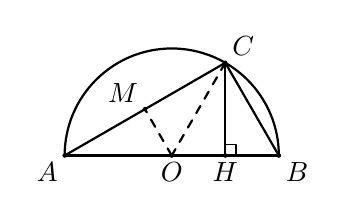
\begin{tikzpicture}[scale=0.68, >=stealth, line join=round, line cap=round]
  \coordinate (A) at (-2, 0);
  \coordinate (B) at (2, 0);
  \coordinate (O) at (0, 0);
  \coordinate (C) at (1, 1.732);
  \coordinate (H) at (1, 0);
  \coordinate (M) at (-0.5, 0.866);
  \draw[thick] (-2, 0) -- (2, 0);
  \draw[thick] (2, 0) arc (0:180:2);
  \draw[thick] (-2, 0) -- (1, 1.732) -- (2, 0);
  \draw[thick] (1, 1.732) -- (1, 0);
  \draw[thick, dashed] (0, 0) -- (-0.5, 0.866);
  \draw[thick, dashed] (1, 1.732) -- (0, 0);
  \draw (1, 0.2) -- (1.2, 0.2) -- (1.2, 0);
  \fill (A) circle (1.2pt) node[below left=-1pt] {$A$};
  \fill (B) circle (1.2pt) node[below right=-1pt] {$B$};
  \fill (O) circle (1.2pt) node[below=-1pt] {$O$};
  \fill (C) circle (1.2pt) node[above right=-1pt] {$C$};
  \fill (H) circle (1.2pt) node[below=-1pt] {$H$};
  \fill (M) circle (1.2pt) node[above left=-1pt] {$M$};
\end{tikzpicture}
\end{minipage}\par
\vspace{0.4mm}
\noindent\textit{Bài giải:}\dongke{16}
\\ \hline
\end{tabularx}

\newpage
% =============================================================================
% ========================= TOAN 9 TUAN 09 BUOI 02 - MA DE 102 =================
% ========================= TRANG 1/2 ==========================================
% =============================================================================
\noindent
\begin{tabularx}{\linewidth}{|X|c|}
\hline
\textbf{PHIẾU KIỂM TRA ĐỊNH KỲ TOÁN 9 - TUẦN 09 - BUỔI 02} & \textbf{Mã đề: 102 - Trang 1/2} \\
\hline
\end{tabularx}

\vspace{1.0mm}

\noindent
\begin{tabularx}{\linewidth}{|p{3.2cm}|X|}
\hline
\centering\textbf{ĐIỂM SỐ} & \centering\textbf{LỜI NHẬN XÉT CỦA THẦY CÔ} \tabularnewline
\hline
\rule{0pt}{1.8cm} & \tabularnewline
\hline
\end{tabularx}

\vspace{1.2mm}
\noindent\textbf{Câu 1 (0,25 điểm).} Tâm đối xứng của đường tròn $(I; R)$ là điểm nào?: \shortans{Tâm I}\par\vspace{0.6mm}
\noindent\textbf{Câu 2 (0,25 điểm).} Số trục đối xứng của một đường tròn là bao nhiêu?: \shortans{Vô số}\par\vspace{0.6mm}
\noindent\textbf{Câu 3 (0,25 điểm).} Đường kính đi qua trung điểm của một dây không đi qua tâm thì: \shortans{Vuông góc với dây}\par\vspace{0.6mm}
\noindent\textbf{Câu 4 (0,25 điểm).} Cho $(O; 10\text{ cm})$, dây $AB = 12\text{ cm}$. Khoảng cách từ tâm $O$ đến dây $AB$ là: \shortans{8\text{ cm}}\par\vspace{0.6mm}
\noindent\textbf{Câu 5 (0,25 điểm).} Cho $(O; 5\text{ cm})$, khoảng cách từ tâm $O$ đến dây $CD$ là $4\text{ cm}$. Dây $CD$ dài: \shortans{6\text{ cm}}\par\vspace{0.6mm}
\noindent\textbf{Câu 6 (0,25 điểm).} Kết quả rút gọn biểu thức $\sqrt{(\sqrt{5} - 2)^2}$ bằng: \shortans{\sqrt{5}-2}\par\vspace{0.6mm}
\noindent\textbf{Câu 7 (0,25 điểm).} Trục căn thức ở mẫu của biểu thức $\dfrac{3}{\sqrt{5}-\sqrt{2}}$ được kết quả là: \shortans{\sqrt{5}+\sqrt{2}}\par\vspace{0.6mm}
\noindent\textbf{Câu 8 (0,25 điểm).} Nghiệm của phương trình $\sqrt{x - 2} = 5$ là $x = $: \shortans{27}\par\vspace{0.6mm}
\noindent\textbf{Câu 9 (0,25 điểm).} Nghiệm của hệ phương trình $\begin{cases} 3x + 2y = 8 \\ 3x - 2y = 4 \end{cases}$ là $(x; y) = $: \shortans{(2; 1)}\par\vspace{0.6mm}
\noindent\textbf{Câu 10 (0,25 điểm).} Vòm tròn bán kính $5\text{ m}$. Bề rộng mặt đường cách đỉnh vòm $2\text{ m}$ là: \shortans{8\text{ m}}\par\vspace{0.6mm}
\vspace{0.8mm}
\noindent\textbf{Câu 11 (2,5 điểm). Đại số tổng hợp:}
\vspace{0.6mm}

\noindent
\begin{tabularx}{\linewidth}{|X|X|}
\hline
\oBaiTap[20]{a) (1,25 điểm)}{Giải hệ phương trình:\par $\begin{cases} 2(x + 1) + 3y = 9 \\ 3x - (y + 2) = 3 \end{cases}$} & 
\oBaiTap[20]{b) (1,25 điểm)}{Cho biểu thức với $x > 0, x \ne 4$:\par $Q = \left(\dfrac{\sqrt{x}+2}{\sqrt{x}-2} - \dfrac{\sqrt{x}-2}{\sqrt{x}+2}\right) : \dfrac{8\sqrt{x}}{x-4}$\par Rút gọn biểu thức $Q$.} \\
\hline
\end{tabularx}

\newpage
% =============================================================================
% ========================= TOAN 9 TUAN 09 BUOI 02 - MA DE 102 =================
% ========================= TRANG 2/2 ==========================================
% =============================================================================
\noindent
\begin{tabularx}{\linewidth}{|X|c|}
\hline
\textbf{TOÁN 9 - TUẦN 09 - BUỔI 02} & \textbf{Mã đề: 102 - Trang 2/2} \\
\hline
\end{tabularx}

\vspace{1.2mm}

\noindent
\begin{tabularx}{\linewidth}{|X|}
\hline
\vspace{0.5mm}
\textbf{Câu 12 (2,5 điểm).} Hai ô tô khởi hành cùng một lúc từ hai địa điểm $A$ và $B$ cách nhau $200\text{ km}$, đi ngược chiều nhau và gặp nhau sau $2$ giờ. Biết rằng vận tốc của ô tô đi từ $A$ lớn hơn vận tốc của ô tô đi từ $B$ là $20\text{ km/h}$. Tính vận tốc của mỗi ô tô.\par
\vspace{0.4mm}
\noindent\textit{Bài giải:}\dongke{16}
\\ \hline
\end{tabularx}

\vspace{1.2mm}

\noindent
\begin{tabularx}{\linewidth}{|X|}
\hline
\vspace{0.5mm}
\begin{minipage}[t]{0.64\linewidth}
\vspace{0pt}
\textbf{Câu 13 (2,5 điểm).} Cho nửa đường tròn $(O; R)$ có đường kính $AB = 10\text{ cm}$. Lấy điểm $C$ thuộc nửa đường tròn sao cho $AC = 8\text{ cm}$ ($C \ne A, C \ne B$). Kẻ $CH \perp AB$ tại $H$ ($H \in AB$).\par\vspace{0.4mm}
\textbf{a) (1,5 điểm)} Chứng minh $\Delta ABC$ vuông tại $C$. Tính độ dài $BC, CH$ và khoảng cách từ tâm $O$ đến dây $AC$.\par\vspace{0.4mm}
\textbf{b) (1,0 điểm)} Gọi $M$ là trung điểm của $AC$. Chứng minh $OM \perp AC$ và $4$ điểm $C, H, O, M$ cùng thuộc một đường tròn.
\end{minipage}\hfill
\begin{minipage}[t]{0.34\linewidth}
\vspace{0pt}\centering
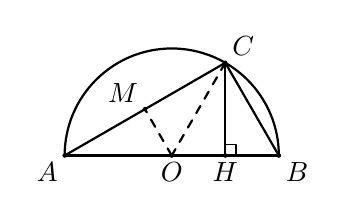
\begin{tikzpicture}[scale=0.68, >=stealth, line join=round, line cap=round]
  \coordinate (A) at (-2, 0);
  \coordinate (B) at (2, 0);
  \coordinate (O) at (0, 0);
  \coordinate (C) at (1, 1.732);
  \coordinate (H) at (1, 0);
  \coordinate (M) at (-0.5, 0.866);
  \draw[thick] (-2, 0) -- (2, 0);
  \draw[thick] (2, 0) arc (0:180:2);
  \draw[thick] (-2, 0) -- (1, 1.732) -- (2, 0);
  \draw[thick] (1, 1.732) -- (1, 0);
  \draw[thick, dashed] (0, 0) -- (-0.5, 0.866);
  \draw[thick, dashed] (1, 1.732) -- (0, 0);
  \draw (1, 0.2) -- (1.2, 0.2) -- (1.2, 0);
  \fill (A) circle (1.2pt) node[below left=-1pt] {$A$};
  \fill (B) circle (1.2pt) node[below right=-1pt] {$B$};
  \fill (O) circle (1.2pt) node[below=-1pt] {$O$};
  \fill (C) circle (1.2pt) node[above right=-1pt] {$C$};
  \fill (H) circle (1.2pt) node[below=-1pt] {$H$};
  \fill (M) circle (1.2pt) node[above left=-1pt] {$M$};
\end{tikzpicture}
\end{minipage}\par
\vspace{0.4mm}
\noindent\textit{Bài giải:}\dongke{16}
\\ \hline
\end{tabularx}

\newpage
% =============================================================================
% ========================= TOAN 9 TUAN 09 BUOI 02 - MA DE 103 =================
% ========================= TRANG 1/2 ==========================================
% =============================================================================
\noindent
\begin{tabularx}{\linewidth}{|X|c|}
\hline
\textbf{PHIẾU KIỂM TRA ĐỊNH KỲ TOÁN 9 - TUẦN 09 - BUỔI 02} & \textbf{Mã đề: 103 - Trang 1/2} \\
\hline
\end{tabularx}

\vspace{1.0mm}

\noindent
\begin{tabularx}{\linewidth}{|p{3.2cm}|X|}
\hline
\centering\textbf{ĐIỂM SỐ} & \centering\textbf{LỜI NHẬN XÉT CỦA THẦY CÔ} \tabularnewline
\hline
\rule{0pt}{1.8cm} & \tabularnewline
\hline
\end{tabularx}

\vspace{1.2mm}
\noindent\textbf{Câu 1 (0,25 điểm).} Tâm đối xứng của đường tròn $(O)$ là điểm nào?: \shortans{Tâm O}\par\vspace{0.6mm}
\noindent\textbf{Câu 2 (0,25 điểm).} Đường thẳng nào sau đây là trục đối xứng của đường tròn?: \shortans{Đường thẳng qua tâm}\par\vspace{0.6mm}
\noindent\textbf{Câu 3 (0,25 điểm).} Dây lớn nhất của đường tròn đi qua điểm nào?: \shortans{Tâm}\par\vspace{0.6mm}
\noindent\textbf{Câu 4 (0,25 điểm).} Cho $(O; 13\text{ cm})$, dây $AB = 24\text{ cm}$. Khoảng cách từ tâm $O$ đến dây $AB$ là: \shortans{5\text{ cm}}\par\vspace{0.6mm}
\noindent\textbf{Câu 5 (0,25 điểm).} Cho $(O; 13\text{ cm})$, khoảng cách từ tâm $O$ đến dây $CD$ là $12\text{ cm}$. Dây $CD$ dài: \shortans{10\text{ cm}}\par\vspace{0.6mm}
\noindent\textbf{Câu 6 (0,25 điểm).} Kết quả rút gọn biểu thức $\sqrt{(\sqrt{10} - 3)^2}$ bằng: \shortans{\sqrt{10}-3}\par\vspace{0.6mm}
\noindent\textbf{Câu 7 (0,25 điểm).} Trục căn thức ở mẫu của biểu thức $\dfrac{4}{\sqrt{5}-1}$ được kết quả là: \shortans{\sqrt{5}+1}\par\vspace{0.6mm}
\noindent\textbf{Câu 8 (0,25 điểm).} Nghiệm của phương trình $\sqrt{x - 5} = 3$ là $x = $: \shortans{14}\par\vspace{0.6mm}
\noindent\textbf{Câu 9 (0,25 điểm).} Nghiệm của hệ phương trình $\begin{cases} 4x + y = 9 \\ 4x - y = 7 \end{cases}$ là $(x; y) = $: \shortans{(2; 1)}\par\vspace{0.6mm}
\noindent\textbf{Câu 10 (0,25 điểm).} Bánh xe có bán kính $0{,}35\text{ m}$. Chu vi bánh xe là (lấy $\pi \approx \frac{22}{7}$): \shortans{2{,}2\text{ m}}\par\vspace{0.6mm}
\vspace{0.8mm}
\noindent\textbf{Câu 11 (2,5 điểm). Đại số tổng hợp:}
\vspace{0.6mm}

\noindent
\begin{tabularx}{\linewidth}{|X|X|}
\hline
\oBaiTap[20]{a) (1,25 điểm)}{Giải hệ phương trình:\par $\begin{cases} 2(x - 1) + y = 3 \\ 3x - 2(y + 1) = 2 \end{cases}$} & 
\oBaiTap[20]{b) (1,25 điểm)}{Cho biểu thức với $x > 0, x \ne 9$:\par $Q = \left(\dfrac{\sqrt{x}+3}{\sqrt{x}-3} - \dfrac{\sqrt{x}-3}{\sqrt{x}+3}\right) : \dfrac{12\sqrt{x}}{x-9}$\par Rút gọn biểu thức $Q$.} \\
\hline
\end{tabularx}

\newpage
% =============================================================================
% ========================= TOAN 9 TUAN 09 BUOI 02 - MA DE 103 =================
% ========================= TRANG 2/2 ==========================================
% =============================================================================
\noindent
\begin{tabularx}{\linewidth}{|X|c|}
\hline
\textbf{TOÁN 9 - TUẦN 09 - BUỔI 02} & \textbf{Mã đề: 103 - Trang 2/2} \\
\hline
\end{tabularx}

\vspace{1.2mm}

\noindent
\begin{tabularx}{\linewidth}{|X|}
\hline
\vspace{0.5mm}
\textbf{Câu 12 (2,5 điểm).} Hai ô tô khởi hành cùng một lúc từ hai tỉnh $A$ và $B$ cách nhau $210\text{ km}$, đi ngược chiều nhau và gặp nhau sau $3$ giờ. Biết rằng vận tốc của ô tô đi từ $A$ lớn hơn vận tốc của ô tô đi từ $B$ là $10\text{ km/h}$. Tính vận tốc của mỗi ô tô.\par
\vspace{0.4mm}
\noindent\textit{Bài giải:}\dongke{16}
\\ \hline
\end{tabularx}

\vspace{1.2mm}

\noindent
\begin{tabularx}{\linewidth}{|X|}
\hline
\vspace{0.5mm}
\begin{minipage}[t]{0.64\linewidth}
\vspace{0pt}
\textbf{Câu 13 (2,5 điểm).} Cho nửa đường tròn $(O; R)$ có đường kính $AB = 20\text{ cm}$. Lấy điểm $C$ thuộc nửa đường tròn sao cho $AC = 12\text{ cm}$ ($C \ne A, C \ne B$). Kẻ $CH \perp AB$ tại $H$ ($H \in AB$).\par\vspace{0.4mm}
\textbf{a) (1,5 điểm)} Chứng minh $\Delta ABC$ vuông tại $C$. Tính độ dài $BC, CH$ và khoảng cách từ tâm $O$ đến dây $AC$.\par\vspace{0.4mm}
\textbf{b) (1,0 điểm)} Gọi $M$ là trung điểm của $AC$. Chứng minh $OM \perp AC$ và $4$ điểm $C, H, O, M$ cùng thuộc một đường tròn.
\end{minipage}\hfill
\begin{minipage}[t]{0.34\linewidth}
\vspace{0pt}\centering
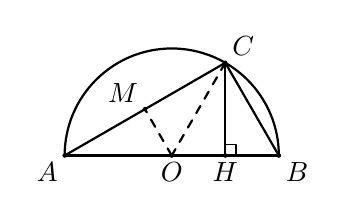
\begin{tikzpicture}[scale=0.68, >=stealth, line join=round, line cap=round]
  \coordinate (A) at (-2, 0);
  \coordinate (B) at (2, 0);
  \coordinate (O) at (0, 0);
  \coordinate (C) at (1, 1.732);
  \coordinate (H) at (1, 0);
  \coordinate (M) at (-0.5, 0.866);
  \draw[thick] (-2, 0) -- (2, 0);
  \draw[thick] (2, 0) arc (0:180:2);
  \draw[thick] (-2, 0) -- (1, 1.732) -- (2, 0);
  \draw[thick] (1, 1.732) -- (1, 0);
  \draw[thick, dashed] (0, 0) -- (-0.5, 0.866);
  \draw[thick, dashed] (1, 1.732) -- (0, 0);
  \draw (1, 0.2) -- (1.2, 0.2) -- (1.2, 0);
  \fill (A) circle (1.2pt) node[below left=-1pt] {$A$};
  \fill (B) circle (1.2pt) node[below right=-1pt] {$B$};
  \fill (O) circle (1.2pt) node[below=-1pt] {$O$};
  \fill (C) circle (1.2pt) node[above right=-1pt] {$C$};
  \fill (H) circle (1.2pt) node[below=-1pt] {$H$};
  \fill (M) circle (1.2pt) node[above left=-1pt] {$M$};
\end{tikzpicture}
\end{minipage}\par
\vspace{0.4mm}
\noindent\textit{Bài giải:}\dongke{16}
\\ \hline
\end{tabularx}

\newpage
% =============================================================================
% ========================= TOAN 9 TUAN 09 BUOI 02 - MA DE 104 =================
% ========================= TRANG 1/2 ==========================================
% =============================================================================
\noindent
\begin{tabularx}{\linewidth}{|X|c|}
\hline
\textbf{PHIẾU KIỂM TRA ĐỊNH KỲ TOÁN 9 - TUẦN 09 - BUỔI 02} & \textbf{Mã đề: 104 - Trang 1/2} \\
\hline
\end{tabularx}

\vspace{1.0mm}

\noindent
\begin{tabularx}{\linewidth}{|p{3.2cm}|X|}
\hline
\centering\textbf{ĐIỂM SỐ} & \centering\textbf{LỜI NHẬN XÉT CỦA THẦY CÔ} \tabularnewline
\hline
\rule{0pt}{1.8cm} & \tabularnewline
\hline
\end{tabularx}

\vspace{1.2mm}
\noindent\textbf{Câu 1 (0,25 điểm).} Số tâm đối xứng của một đường tròn là bao nhiêu?: \shortans{1}\par\vspace{0.6mm}
\noindent\textbf{Câu 2 (0,25 điểm).} Mỗi đường kính của một đường tròn có là trục đối xứng không?: \shortans{Có}\par\vspace{0.6mm}
\noindent\textbf{Câu 3 (0,25 điểm).} Dây không đi qua tâm thì luôn có độ dài so với đường kính như thế nào?: \shortans{Nhỏ hơn}\par\vspace{0.6mm}
\noindent\textbf{Câu 4 (0,25 điểm).} Cho $(O; 15\text{ cm})$, dây $AB = 24\text{ cm}$. Khoảng cách từ tâm $O$ đến dây $AB$ là: \shortans{9\text{ cm}}\par\vspace{0.6mm}
\noindent\textbf{Câu 5 (0,25 điểm).} Cho $(O; 17\text{ cm})$, khoảng cách từ tâm $O$ đến dây $CD$ là $15\text{ cm}$. Dây $CD$ dài: \shortans{16\text{ cm}}\par\vspace{0.6mm}
\noindent\textbf{Câu 6 (0,25 điểm).} Kết quả rút gọn biểu thức $\sqrt{(4 - \sqrt{15})^2}$ bằng: \shortans{4 - \sqrt{15}}\par\vspace{0.6mm}
\noindent\textbf{Câu 7 (0,25 điểm).} Trục căn thức ở mẫu của biểu thức $\dfrac{2}{\sqrt{5}-\sqrt{3}}$ được kết quả là: \shortans{\sqrt{5}+\sqrt{3}}\par\vspace{0.6mm}
\noindent\textbf{Câu 8 (0,25 điểm).} Nghiệm của phương trình $\sqrt{x - 7} = 4$ là $x = $: \shortans{23}\par\vspace{0.6mm}
\noindent\textbf{Câu 9 (0,25 điểm).} Nghiệm của hệ phương trình $\begin{cases} 5x + 2y = 12 \\ 5x - 2y = 8 \end{cases}$ là $(x; y) = $: \shortans{(2; 1)}\par\vspace{0.6mm}
\noindent\textbf{Câu 10 (0,25 điểm).} Đĩa tròn có bán kính $14\text{ cm}$. Chu vi đĩa tròn là (lấy $\pi \approx \frac{22}{7}$): \shortans{88\text{ cm}}\par\vspace{0.6mm}
\vspace{0.8mm}
\noindent\textbf{Câu 11 (2,5 điểm). Đại số tổng hợp:}
\vspace{0.6mm}

\noindent
\begin{tabularx}{\linewidth}{|X|X|}
\hline
\oBaiTap[20]{a) (1,25 điểm)}{Giải hệ phương trình:\par $\begin{cases} 4(x - 1) + 3y = 7 \\ 2x - (y + 1) = 2 \end{cases}$} & 
\oBaiTap[20]{b) (1,25 điểm)}{Cho biểu thức với $x > 0, x \ne 16$:\par $Q = \left(\dfrac{\sqrt{x}+4}{\sqrt{x}-4} - \dfrac{\sqrt{x}-4}{\sqrt{x}+4}\right) : \dfrac{16\sqrt{x}}{x-16}$\par Rút gọn biểu thức $Q$.} \\
\hline
\end{tabularx}

\newpage
% =============================================================================
% ========================= TOAN 9 TUAN 09 BUOI 02 - MA DE 104 =================
% ========================= TRANG 2/2 ==========================================
% =============================================================================
\noindent
\begin{tabularx}{\linewidth}{|X|c|}
\hline
\textbf{TOÁN 9 - TUẦN 09 - BUỔI 02} & \textbf{Mã đề: 104 - Trang 2/2} \\
\hline
\end{tabularx}

\vspace{1.2mm}

\noindent
\begin{tabularx}{\linewidth}{|X|}
\hline
\vspace{0.5mm}
\textbf{Câu 12 (2,5 điểm).} Hai ô tô khởi hành cùng một lúc từ hai tỉnh $A$ và $B$ cách nhau $240\text{ km}$, đi ngược chiều nhau và gặp nhau sau $3$ giờ. Biết rằng vận tốc của ô tô đi từ $A$ lớn hơn vận tốc của ô tô đi từ $B$ là $20\text{ km/h}$. Tính vận tốc của mỗi ô tô.\par
\vspace{0.4mm}
\noindent\textit{Bài giải:}\dongke{16}
\\ \hline
\end{tabularx}

\vspace{1.2mm}

\noindent
\begin{tabularx}{\linewidth}{|X|}
\hline
\vspace{0.5mm}
\begin{minipage}[t]{0.64\linewidth}
\vspace{0pt}
\textbf{Câu 13 (2,5 điểm).} Cho nửa đường tròn $(O; R)$ có đường kính $AB = 20\text{ cm}$. Lấy điểm $C$ thuộc nửa đường tròn sao cho $AC = 16\text{ cm}$ ($C \ne A, C \ne B$). Kẻ $CH \perp AB$ tại $H$ ($H \in AB$).\par\vspace{0.4mm}
\textbf{a) (1,5 điểm)} Chứng minh $\Delta ABC$ vuông tại $C$. Tính độ dài $BC, CH$ và khoảng cách từ tâm $O$ đến dây $AC$.\par\vspace{0.4mm}
\textbf{b) (1,0 điểm)} Gọi $M$ là trung điểm của $AC$. Chứng minh $OM \perp AC$ và $4$ điểm $C, H, O, M$ cùng thuộc một đường tròn.
\end{minipage}\hfill
\begin{minipage}[t]{0.34\linewidth}
\vspace{0pt}\centering
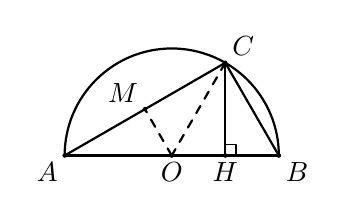
\begin{tikzpicture}[scale=0.68, >=stealth, line join=round, line cap=round]
  \coordinate (A) at (-2, 0);
  \coordinate (B) at (2, 0);
  \coordinate (O) at (0, 0);
  \coordinate (C) at (1, 1.732);
  \coordinate (H) at (1, 0);
  \coordinate (M) at (-0.5, 0.866);
  \draw[thick] (-2, 0) -- (2, 0);
  \draw[thick] (2, 0) arc (0:180:2);
  \draw[thick] (-2, 0) -- (1, 1.732) -- (2, 0);
  \draw[thick] (1, 1.732) -- (1, 0);
  \draw[thick, dashed] (0, 0) -- (-0.5, 0.866);
  \draw[thick, dashed] (1, 1.732) -- (0, 0);
  \draw (1, 0.2) -- (1.2, 0.2) -- (1.2, 0);
  \fill (A) circle (1.2pt) node[below left=-1pt] {$A$};
  \fill (B) circle (1.2pt) node[below right=-1pt] {$B$};
  \fill (O) circle (1.2pt) node[below=-1pt] {$O$};
  \fill (C) circle (1.2pt) node[above right=-1pt] {$C$};
  \fill (H) circle (1.2pt) node[below=-1pt] {$H$};
  \fill (M) circle (1.2pt) node[above left=-1pt] {$M$};
\end{tikzpicture}
\end{minipage}\par
\vspace{0.4mm}
\noindent\textit{Bài giải:}\dongke{16}
\\ \hline
\end{tabularx}
\end{document}
